\chapter{Theory and Literature Review}
Modelling for the storage of BOS filter cake within stockpiles does not exist within the literature. The material is specific to the industry and presents its own challenges. In order to build appropriate models we utilise work conducted in existing industrial applications. We need to combine these models with the experimental data in order to provide useful models for stockpile ignition.

\section{Experimental work}
Experimental work has been conducted by Longbottom et al. \cite{Ray19} to evaluate the effectiveness of the filter cake to improve its recyclability. Through understanding the experimental work, we can use models to simulate the results and use the experimental data to fit these models. These experimental models can be used to develop more effective predictions in the larger stockpiles that we are interested in.

\subsection{Characterisation of the Material}
A key aspect of this thesis is the material used to build these stockpiles. The results from Longbottom et al. \cite{Ray19} determined the composition of the filter cake as well as the composition after some reactions had taken place. The important aspects of composition for this thesis, is the mass percentage of metallic iron and W\"{u}stite, 16.9\% and 29.8\% respectively. 
\subsection{Experimental Procedures}
One of the facets about this research project is the availability of experimental data. This allows more complicated models to be developed, as more parameters can be determined from experimental data. An additional benefit is that the models can be tested on smaller scales, to assess the accuracy. The relevant experimental techniques need to be understood in order to be able to model what is occurring.
%for more complicated models to be developed, as relevant data can be measured, though this requires a more thorough understanding of the experimental techniques and the relevant theory. 

\subsubsection{Thermogravemetric Analysis}
Thermogravemetric analysis (TGA), measures the weight change of a sample. A small sample is heated, usually at a fixed rate, and any deviation in mass is recorded. The technique is useful for assessing reactions such as oxidation and vaporisation, which have been observed from the experimental data for the filter cake \cite{Ray19}. Reactions such as melting and crystallisation cannot be investigated as the mass of the sample does not change \cite{thermal}.\\

In a small scale TGA experiment a 100 mg sample is placed in a crucible that is attached to a balance. Air is fed through the base of the set-up, and the sample is heated at a fixed rate via radiative heating. As the sample undergoes reactions the weight change is measured.\\

This set-up can be changed to include larger sample sizes, though this affects the quality of the data. With larger samples, significant temperature gradients within the sample can occur; as a result, diffusion needs to be considered and heating at a fixed rate becomes more difficult. Since the sample is larger, it can be representative of the stockpiled material. Having a bigger sample also improves the repeatability of the experiment.\\
\begin{figure}[h!]
\centering
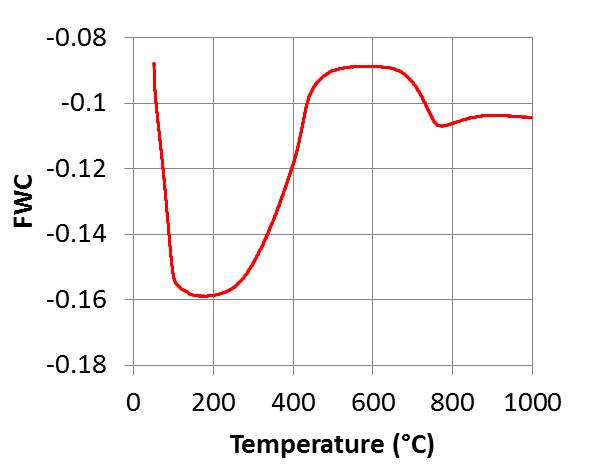
\includegraphics[scale=1]{figures/TGA_exp.jpg}
\caption{The Fractional weight change curve obtained from the TGA experiment \cite{Ray19}.}
\label{TGA_exp}
\end{figure} 
\subsubsection{Differential Scanning Calorimetry}
The set-up of the differential scanning calorimetry (DSC) is similar to that of the TGA. The experimental procedure of heating the sample is the same and as a result the two experiments can be conducted simultaneously. DSC however measures the heat of the reactions occurring in the sample. This is done by measuring temperature differences\cite{thermal}.\\  
\begin{figure}
\centering
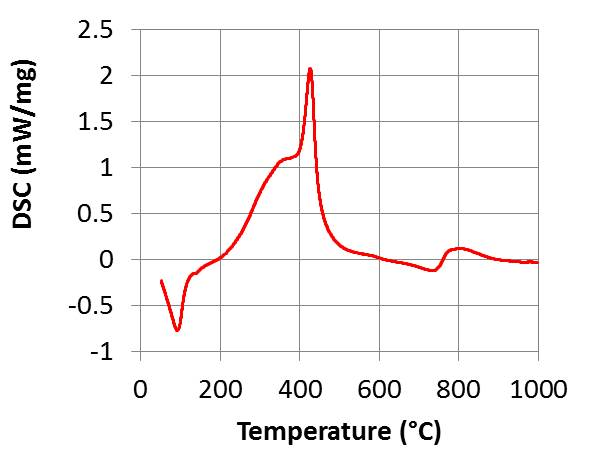
\includegraphics[scale=1]{figures/DSC_exp.jpg}
\caption{The DSC curve obtained through experimentation \cite{Ray19}.}
\label{DSC_exp}
\end{figure} 

\section{Frank Kamentskii Theory}
The fundamental theory of spontaneous combustion, is known as Frank-Kamentskii theory \cite{bowes}. The theory is based around temperature diffusion with an Arrhenius reaction term. The equation is,
\begin{equation}
\rho c\frac{\partial T}{\partial t}=k\frac{\partial^2 T}{\partial x^2}+Q\rho A\exp\left(\frac{-E}{RT}\right). \label{Comb_model}
\end{equation}
It is useful to consider the steady state solution of this equation.  
%include the scaled variables as well.
After rescaling the variables the steady state solution solves the differential equation,
\begin{equation}
\frac{d^2u}{dz^2}=-\delta\exp\left(\frac{u}{1+\varepsilon u}\right). \label{FK_mod}
\end{equation}
Using the Frank-Kamentskii approximation $\eps=0$, an analytic solution to the equation can be derived. This equation is the 1-dimensional analogue of Semenov's condition for ignition in a self-heating system \cite{bowes}.  The existence of this solution is dependant on the value for $\delta$ with two solutions existing for $\delta<\delta_{cr}$ \cite{bowes}. A large amount of combustion modelling uses this critical condition as a means of developing an ignition criteria for the stockpiles.
\subsection{Application to stockpile Ignition}
The model described in equation \eqref{Comb_model} has been used in a range of industries including oxidative heating, in materials such as coal and biological heating that occurs during composting \cite{bowes}. In each of these applications there are slight differences in how the theory is applied. 
\subsubsection{Compost}
In the composting process the method of heating cannot simply be taken as an Arrhenious reaction. Instead a second heating function is required to model the microbial heating.  Nelson et al.\cite{NELS03} proposed the following model,
\begin{multline}
\rho c_vV\frac{dT}{dt}=Q_bVF_b\frac{A_1\exp[-E_1/RT]}{1+A_2\exp[-E_2/RT]}B\left(1-\frac{B}{B_{max}}\right)+Q_cVA_3\exp\left[\frac{-E_3}{RT}\right]C\\-\chi S\left(T-T_a\right). \label{Bio}
\end{multline}
This has been used as a basis for much of the following work involving compost models. This model has been extended to a two-dimensional model with temperature diffusion \cite{sidhu06}. This latter model can be used to determine a critical ignition length for a stockpile.\\
An extension of this model is to introduce oxygen into the spatially uniform models \cite{nels07}.
The consumption of oxygen limits the reaction, and consequently the temperature. This base model has been extended into two dimensions with diffusion of oxygen \cite{Sidhu2007}.\\
When extending to multiple dimensions, an airflow is also added into the equations.
In the one dimensional case, airflow can only be considered in one direction \cite{luang09,luang10}. When in two dimensions, an equation is required to express the airflow through the stockpile. This is done as a forced flow where the airflow is independant of temperature \cite{luang10b,luang10c}. Aganetti et al. \cite{aga16} used a Darcy-Brinkman equation for flow in a porous medium. The airflow inside these stockpiles have been studied further with different flows able to be described. \cite{AGA17}\\
The  effect of moisture on the reaction has also been added into the model \cite{ZAM11,luang18,luang11a}. When modelling the moisture content, both a liquid water concentration and a water vapour concentration are needed. The concentration of liquid water affects the reaction rate; at higher water levels, there is an increased coverage of the reaction sites. The effects of ambient humidity, on the ignition criteria has been investigated \cite{luang18u} \\
Further additions to the model have been to consider different geometries \cite{luang11a} and also to use radiative boundary conditions \cite{luang10d,MOR09}. These developments add more complexities into the model but improves its accuracy.\\
%\subsubsection{Coal}
Many of the developments to these models can be adapted and applied to filter cake stockpiles. There are some key points where the two problems differentiate, one of which is the construction of the stockpiles. The stockpiles are built up gradually over time and this has to be taken into account. The compost models focus on preventing combustion, so when the stockpile is increased in size, a cautious approach would be to consider fresh compost. This will underestimate the critical combustion length. The need for a model that considers a changing domain is dependant on the consumption of reactants due to this.

\subsubsection{Coal}
Coal stockpiles have also been modelled using the FK framework \cite{Zhang16}. 
\subsubsection{Periodic Boundary conditions}
The basic model can be adapted by change the boundary condition. One such method is to have an oscillating ambient temperature. The stockpiles are exposed to diurnal and seasonal temperature variation. Shteinberg and Khudyaev \cite{shtein05} proposed an ODE model, given by,
\begin{align}
\frac{d\theta}{d\tau}&=a\E^\theta-\frac{1}{\delta}\left[\theta-\theta_A\sin\left(\frac{\omega\tau}{\delta}\right)\right],\\
\frac{da}{d\tau}&=-\gamma a\E^\theta,
\end{align}
for the averaged temperature and reactant consumption across the domain. Gorel'skii et al. \cite{gorel10}, analysed this model. These models do not consider the diffusion of temperature, so cannot distinguish regions that have different temperatures. \\
Novozhilov \cite{novozhilov16} proposed a model in one dimension with a single sinusoidal, oscillating boundary. Critical dependencies for the non-dimensionalised amplitude of the oscillations, were developed in terms of the other variables. The analysis was limited to the scaled equations rather than providing any direct application to any problems. Both convective heat transfer and fixed temperature boundary conditions were considered.\\
Novozhilov \cite{novozhilov18} added reactant consumption to the model, using a first order reaction scheme. The effects of having an initial condition that differs from the ambient temperature is also added \cite{novozhilov18}. As more complexities are introduced into the model there are more parameters to investigate. The study similarly determined critical dependencies of the scaled amplitude oscillations. Providing a critical condition for this scaled oscillation amplitude, does provide some insight into the problem, however, it does not address ways to prevent or promote ignition. This parameter does not include variables such as the stockpile length which can be controlled.\\ 
Roy \cite{roy18} proposed a two dimensional model to investigate the effects of oscillating boundary conditions. The proposed model included an oscillating boundary condition along one of it's edges with fixed temperatures on the other edges. It included convection terms, though limited this to a closed system (no air flowing in or out of the domain). As such, the model is more applicable to an experimental set-up, rather than to assess the ignition in large stockpiles where the oscillations are expected on the majority of the boundary.\\ 
We see that there is comparatively limited work with oscillating boundary conditions. The current models proposed are limited in their dimensions and subsequently their application to large stockpiles. The models are restricted to one sinusoidal function, whereas a model including both seasonal and diurnal temperature variation may be more appropriate.
%cite reference for dual sinusoidal weather function.
 It may also be useful to use include the weather data that has been recorded, as this will be more accurate than using a sinusoidal function.

\subsection{Theory applied to experimental work}
\label{Kis}
The models used for thermogravemertic analysis have been reported in studies from Flynn and Wall \cite{flynn66} and Sharp \cite{sharp69}. In these studies the proposed model was in terms of conversion, given,
\begin{equation}
\frac{dC}{dt}=kf(C), \label{fl}
\end{equation}
where k is reaction dependant. In this case the conversion, C, can be expressed as, $C=1-\left(\left(W-W_f\right)/\left(W_0-W_f\right)\right)$, where $W$ is the weight, $W_f$ is the final weight, and $W_0$ is the initial weight. This implies that the initial concentration, $C(0)=0$ The expression for $f(C)$, is dependant on the reaction order. For a reaction of order $n$,
\begin{equation}
f(C)=(1-C)^n.
\end{equation}
This has the effect that for higher concentrations the reaction is accelerated and slows once more of the reactant is consumed. The reaction rate $k$, varies with temperature per an Arrhenious expression, \\
\begin{equation}
k=A\exp\left(\frac{-E}{RT}\right),
\end{equation}
where, A is a pre-exponential rate factor, E is the activation energy, and R is the ideal gas constant.\\
It is not necessary to write the equations in terms of the conversion factor. Ozawa \cite{ozawa65}, uses the weight directly. The equation is,
\begin{equation}
-\frac{dW}{dt}=A\exp\left(\frac{-E}{RT}\right) W^n. \label{oz}
\end{equation} 
It is straightforward to show that these equations are equivalent. This requires equation \eqref{oz}, to be rescaled by the initial weight. In the two equations, the interpretation of the pre-exponential factor is different. This can be seen from dimensional analysis. For equation \eqref{oz}, $\frac{dW}{dt}$ has units $MT^{-1}$, where $M$ is units of mass and $T$ is units of time. As a result $A\exp(E/RT)W^n$ must also have units $MT^{-1}$. The exponential term is dimensionless, and $W^n$ has dimension $M^n$. As a result the dimension of the pre-exponential factor is $M^{1-n}T^{-1}$. For equation \eqref{fl}, there is no mass dimension involved in the equation as we are dealing with the dimensionless conversion factor $C$. The only units involved are time and since the reaction rate $k$ must have units $T^{-1}$, the pre-exponential factor, $A$, must have dimension $T^{-1}$. The units are only the same when the equation is first order, $n=1$. In this case the reaction is invariant under scaling of $W$. It is also useful to note that different reaction order equations have different pre-exponential factors.
The same equations have been used in other studies to evaluate the kinetic parameters A and E \cite{carrasco93,kissinger56,sbirrazzuoli97}.\\
Kissinger \cite{kissinger56} developed a method that can be used to determine the reaction constants, $A$ and $E$. This method was to examine when the reaction rate is at its peak. The reaction rate for Equation \eqref{oz} is at it's maximum when, 
\begin{equation}
\frac{d}{dt}\left(\frac{dW}{dt}\right)=0.
\end{equation}
In the work carried out by Kissinger, it was assumed that the reaction order was one. This resulted in the equation,
\begin{equation}
A\exp\left(\frac{-E}{RT_m}\right)=\frac{E}{RT_m^2}\frac{dT}{dt},
\end{equation}
where $T_m$ is the temperature at which the maximum reaction rate occurs, and $\frac{dT}{dt}=\alpha$, which is the heating rate in the experiment. By taking logarithms straight line equation can be formed, for the variables, $X=1/T_m$ and $Y=\log\left(\alpha/T_M^2\right)$ allowing a linear regression to be performed. If we do not assume the reaction order, then an additional term, the amount of converted material, is required. From this equation the reaction order and the kinetic parameters can be estimated. To estimate the parameters in this way, we must be able to determine the Temperature at which the maximum reaction rate is achieved. With two reactions this is difficult to achieve. This equation is still useful in being able to relate our parameters.\\
%As an aside, for this reaction problem where we have two distinct reactions occurring, determining the converted fraction of material will be difficult. As a result the simplifying assumption is to take a first order reaction.
\subsection{Critical Ignition Criteria}
The Frank-Kamanetskii theory states that for the case when $\delta<\dcr$, there exists a low temperature solution and a high temperature solution \cite{Gray93,bowes}. Various ignition criteria have been investigated. Weber et al \cite{weber98} investigates the effects that different families of initial conditions have. These include, constant, linear and quadratic initial temperature profiles. These initial investigations provided some useful critical ignition conditions though they lack any consumption of material. Brindley, Griffiths and McInstosh \cite{brindley01} address this by introducing consumption and also restricting their analysis to an embedded hotspot. They numerically examinded some criteria required to iniate combustion waves. The existence and propogation of combustion waves have been well studied by various authors \cite{merzhanov88,gubernov12,mcintosh04,weber97,mercer96}. 
McIntosh, Brindley and Griffiths \cite{mcintosh02} futher build upon their work to produce an analytic approach to this problem. This extends previous work that has been done on strongly reactive material \cite{Jackson89,kapila81}. The hotspots examined used a constant power source for their hotspot. For our industrial stockpiles we use a hotspot consisting of previously reacted material.\\

More recent work from Shah et al \cite{shah07} examines hotspots more consistent with the tyoe we are interested in. This research examines the smoldering bahaviour where the reaction rate is controlled by a low oxygen concentration where the reactions are occurring. The key introduction here is the introduction of Oxygen into the model and the subsequent porosity. This theory has been applied to numerical and experimental studies into ignition by a heated particle \cite{wang15,glushkov11}. Similar experimental work has been done by Caine et al \cite{caine10} where they investigated a hotspot with constant power.\\

These studies have developed a lot of theory regarding the ignition of materials using hotspots. One area that appears to be lacking, is the use of previously reacted material. 


\subsection{Parallel Reactions}
Much of the standard approach to Frank-Kamanteskii theory uses a single reaction. The work of Longbottom et al. \cite{Ray19} indicates that we may have several reactions occuring during the sintering process. Boddington et al. \cite{bodd84} developed the foundations of Frank-Kamenetskii theory with parallel reactions. The paper determines a method to calculate an effective activation energy and FK parameter. This then reduces the parallel reactions to a single reaction for which we can apply the existing theory for. Graham-Eagle and Wake \cite{GE85} extended this theory to determine the critical FK parameter in an infinite cylinder and sphere. Graham-Eagle and Wake \cite{GE86} then extend this further to examine the effects of introducing an endothermic reaction. All previous work had only considered exothermic reactions as these are the drivers of self-ignition. This theory has been used to simplify reaction equations in various different contexts and with differing numbers of reactions \cite{wake92,push89,ajadi09,jones91}. \\

Wake et al. \cite{wake92} used this theory to examine heating in forest litter and coal. Pushpavanam and Narayanan \cite{push89} considered the effects of having an endothermic and exothermic reaction in parallel to investigate the ignition and extinction points of the steady state solution. Ajadi and Gol'dshtein \cite{ajadi09} studies the critical behaviour of a three step reaction scheme using this technique.  
 

\subsection{Moisture}
Moisture can be an important factor to consider. There have been instances in the literature \cite{back81,walker67,lohrer05} where wetting of dry material has been found to have caused ignition. Gray and Wake \cite{gray90} models this ignition phenomenon by using a series of parallel reactions. They considered the heat generated through the wetting process and also the cooling effect of evaporation. These two concepts are important to address in investigating our stockpiles. 

\subsubsection{Drying}
Different drying models have been proposed \cite{chen98}. This includes a reaction engineering approach that models evaporation as an Arrhenious expression with activation energy as the latent heat of vaporisation. Similarly condensation is modelled using a zero activation energy assumption. This form of drying was used by Luangwilai \cite{luang11} when investigating how moisture is evaporated in the compost piles.\\
Chen \cite{chen98} proposed a model that looks at evaporation and condensation in terms of an exchange between two surfaces. The change in concentration is proportional to the difference in concentration at the inner surface, and the surface area. Similarly we have a change occurring that is proportional to the concentration difference on the outer surface. The advantage of this approach, is that it considers the concentration of water vapour within the sample, to be distinct from its concentration in ambient air. The issue with this model is that it introduces additional parameters. One of the new terms introduced is the surface area of the small scale particles within the sample. In the context of our material, that does not appear to be a feasible option, as determining the surface area is quite complicated. For simplicity, we therefore use the reaction engineering approach to drying.

\subsubsection{Affect on the reaction}
Characterising how the moisture affects the reaction is not a simple task. We can consider inhibition due to covering the surface available for the reaction. Luangwilai \cite{luang11} used this approach when modelling the combustion of organic material in compost heaps. It was assumed that if the concentration is above a critical concentration, then the reaction would stop. The function is normalised so that when there is no water then the reaction is maximised and the effect of moisture is set to 1. Then the function decreases to 0 as the water concentration approaches some critical concentration. \\
More work needs to be done experimentally to characterise how the moisture levels affect the reaction. From the TGA data provided by Longbottom et al.\cite{Ray19}, it appears as though the reactions are activated at temperatures above the evaporation point of water. This may indicate that the water woould not have any effect as the reactions are not significant at those low temperatures.



\subsection{Radiation effects on Conduction}
The effect of radiation on stockpile ignition is not a common consideration. The modelled stockpiles usually are to prevent ignition \cite{Zhang16}. Mercer and Weber \cite{mercer97} studied the effects of radiative transfer on combustion wave speeds. The radiation effects included was in terms of a radiative heat flux. The net radiative energy emitted and absorbed by the matter per unit time per unit volume is given by $ \nabla \cdot \mathbf{q}^r$, where $\mathbf{q}^r$ is the radiative heat flux  \cite{ozisik73}. The Eddington approximation in one direction is given by the differential equation,
\begin{equation}
\frac{d^2 q^r(\tau)}{d\tau^2}=(1-\omega)\left[4\pi\frac{dI_b(\tau)}{d\tau}+3q^r(\tau)\right],
\end{equation}
where $\omega$ is the albedo, and $I_b(\tau)$ is the total black-body radiation intensity. We can relate the total black-body radiation intensity to the Temperature, 
\begin{equation}
I_b(x)=\frac{\sigma n^2 T(x)^4}{\pi}, \label{black_body}
\end{equation}
where $\sigma$ is the Stefan-Boltzman constant and $n$ is the refractive index. This approximation is for optically thick medium, as a result, this approximation is not as accurate near the boundaries \cite{ozisik73}. In the literature \cite{joulin86,mercer97} the approximation has been altered to,
\begin{equation}
L^2\frac{d^2 q^r(x)}{dx^2}=\left[4\pi L\frac{dI_b(x)}{dx}+3q^r(x)\right],
\end{equation}   
where L is the local absorption length. When the local absorption length is small compared to the length of the medium, then a simplified expression can be used,
\begin{equation}
q^r(x)=-\frac{4\pi}{3} L\frac{dI_b(x)}{dx}.	\label{qr}
\end{equation}
This is the case of optically thick mediums \cite{mercer97}.\\

When incorporating this into the model given by equation \ref{Comb_model} we have, 
\begin{equation}
\rho c\frac{\partial T}{\partial t}=k\frac{\partial^2 T}{\partial x^2}+Q(T)+\frac{\partial q^r}{\partial x}. \label{Rad_model}
\end{equation}
This was investigated by Mercer and Weber \cite{mercer97}. Substituting in equations \ref{black_body} and \ref{qr} and rearranging we obtain,
\begin{equation}
\rho c\frac{\partial T}{\partial t}=\frac{\partial}{\partial x}\left(\left(k-\frac{16}{3} L \sigma n^2 T^3\right)\frac{\partial T}{\partial x}\right) +Q(T).
\end{equation}
This equation provides an effective radiative conductivity, $k_r$ that satisfies $$q^r(x)=-k_r \frac{dT}{dx}$$.

%\section{Ignition of metal powders}

\section{Parameter Estimation}
An important aspect of our modelling is determining the parameter values for the reaction model. Experimental work has been conducted on the BOS filter cake \cite{Ray19,ray20}. We use the TGA and DSC data to fit our model. One of the common approaches is to use that of Kissinger \cite{kissinger56} outlined in section \ref{Kis}. This uses the equation,
\begin{equation}
A\exp\left(\frac{-E}{RT_m}\right)=\frac{E}{RT_m^2}\frac{dT}{dt}, \label{eqkis}
\end{equation}
with different heating rates and corresponding maximum temperatures. Taking logarithms we can rearrange equation \ref{eqkis} to,
\begin{equation}
\log\left(\frac{\alpha}{T_m^2}\right)=\log\left(\frac{AE}{R}\right)-\frac{E}{R}\frac{1}{T_m}.
\end{equation}
This is a straight line for the variables, $X=1/T_m$ and $Y=\log\left(\alpha/{T_m^2}\right)$, allowing a linear regression analysis. This method is not as useful for systems where multiple reactions are occurring. The reason for this is that we cannot determine the temperature at which the reaction rate for each reaction is maximised.\\
Another approach is to use the critical FK parameter, $\delta$. The FK parameter is given by,
\begin{equation}
\delta=\left(\frac{L}{2}\right)^2\frac{QCA}{k}\exp\left(\frac{-E}{RT_a}\right)\frac{E}{RT_a^2}.
\end{equation} 
Taking logarithms we can rearrange this to,
\begin{equation}
\log\left(\frac{4 \delta T_a^2}{L^2}\right)=\log\left(\frac{QCA}{k} \frac{E}{R}\right)-\frac{E}{R}\frac{1}{T_a}. 
\end{equation}
The hot storage test heats a basket of material at a fixed ambient condition. By determining which ambient temperature causes the basket to ignite, for multiple size baskets, we can use a regression model to determine the parameters \cite{gray84}. Jones and Wake \cite{jones90} used this method to determine the kinetic parameters for several materials. This method also has similar issues as it only considers one reaction. Jones \cite{jones92} uses the work of Boddington et al. \cite{bodd84} on parallel reactions to modify this method for two reactions. This adjustment relies on knowing some information that we do not possess. However in our stockpiles the exact reactions have not been determined so those know parameters are not known in our stockpiles.\\

Include two other techniques here mentioned by zanoni.\\

These standard techniques are insufficient to estimate the kinetic parameters when we have multiple reactions. We cannot know what the temperature is which maximises each reaction rate. Another approach is to use an optimisation algorithm. Elliot et al. \cite{elliot05} use a genetic algorithm as an optimasation tool for a system of parallel reactions.  Zanoni et al. \cite{zanoni12} used a Levenberg-Marquardt algorithm to determine the kinetic parameters in a reaction scheme. The objective functions in these cases are complex, exhibiting multiple local minima and maxima, as such gradient based optimisation algorithms are not as successful \cite{elliott05}. Reverte et al. \cite{reverte07} also used a Levenberg-Maraquardt algorithm. They used this to determine an optimal experimental design in order to minimise the error in the parameters estimated. They optimised the design for sample weight, temperature profile, and gas flow rate. The objective fuction minimised was a sum of squares of the measured data and the predicted data.\\
Using these techniques, quantifying the uncertainty in the model becomes more difficult. We use a Markov-Chain Monte-Carlo (MCMC) method to estimate our parameters. An outline of the method is provided in the Appendix. The main advantage of using a MCMC algorithm, is that we are able to draw a sample from the distribution of possible parameter values. We can use this sample to estimate posterior expectations for different quantities including the critical length of the stockpiles. The optimisation based methods allow the variance around the optimum value to be determined, but does not naturally allow a sample to be obtained and parameters to be transformed.\\
The Bayesian approach has been used in recent studies of coal blends \cite{buyu17,buyu17p}. These studies used Monte-Carlo simulations in order to characterise the uncertainty in the predictor coefficients for a multiple non-linear regression analysis. This is a similar idea to our approach, however we assess the uncertainty of parameters in an ODE model.\\

